\section{Systematization of Web3 RegTech}
\label{sec:systematization}

\begin{figure*}[t]
\centering
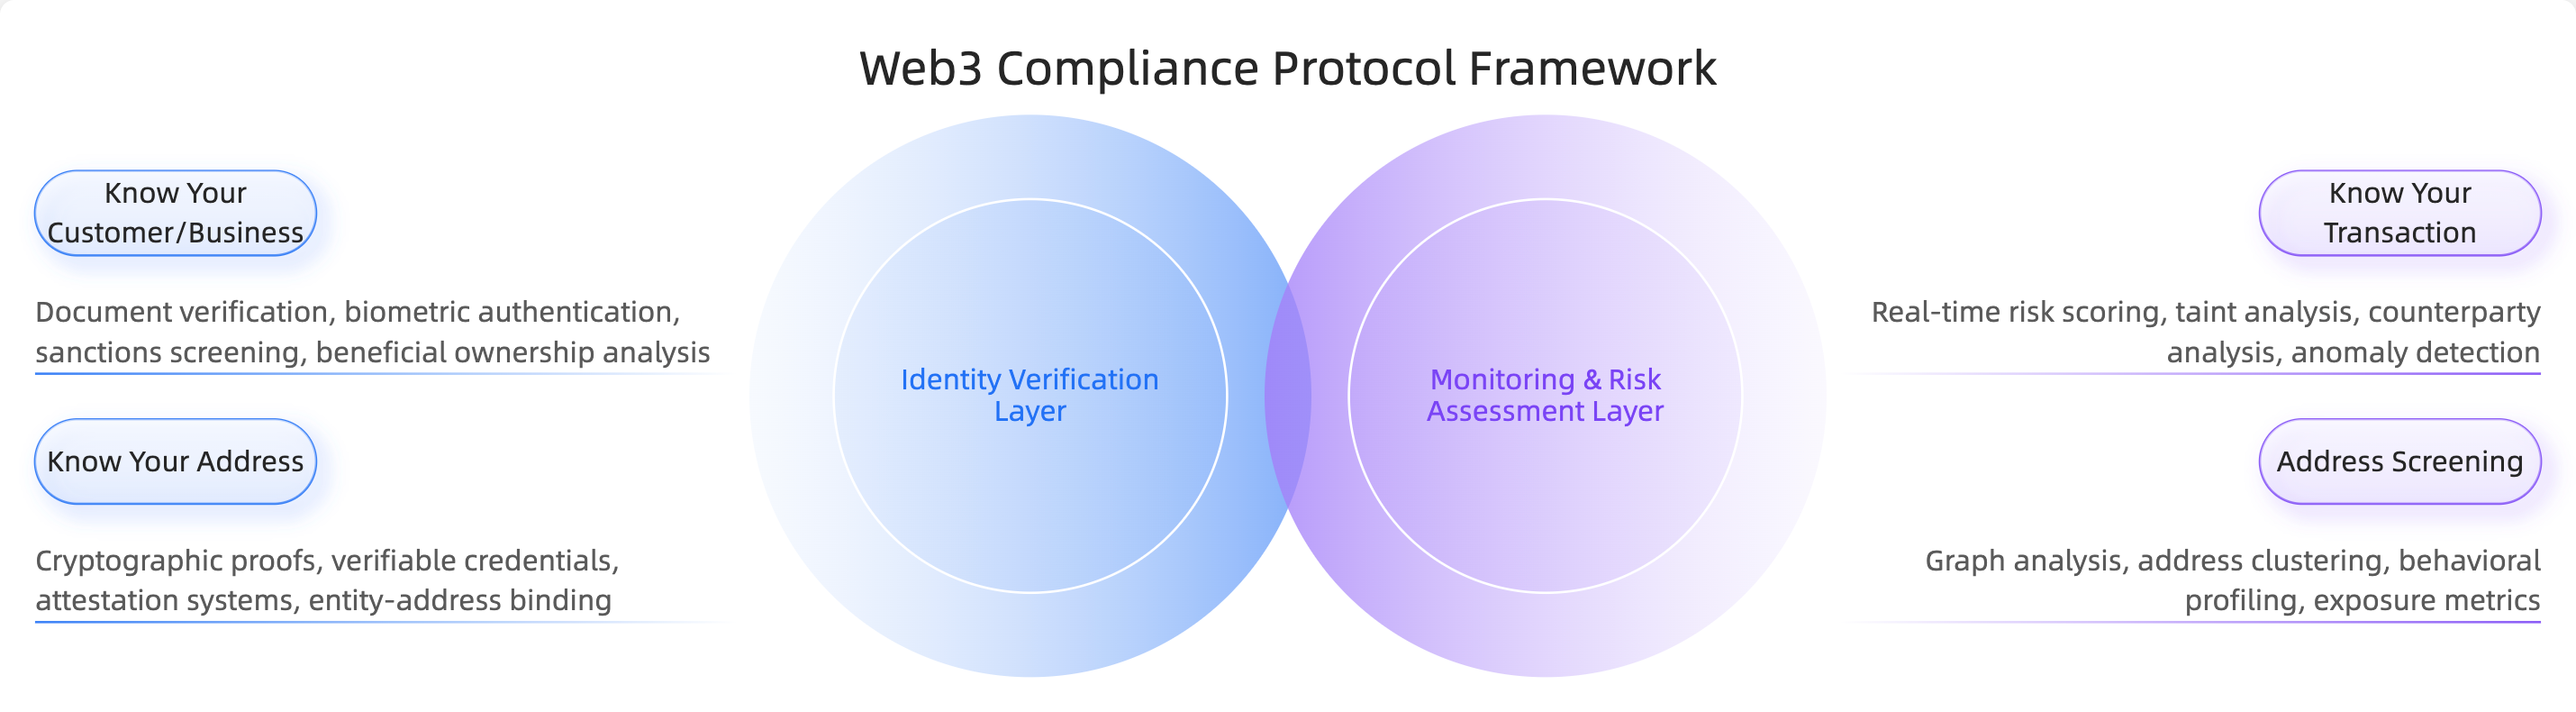
\includegraphics[width=0.95\linewidth]{./compliance-protocol-framework.png}
\caption{Web3 Compliance Protocol Framework: Two-Layer Architecture. This framework organizes compliance protocols into two fundamental layers: (1) Identity Verification Layer establishes and verifies identities across entity level (Know Your Customer/Business) and address level (Know Your Address) through document verification, biometric authentication, sanctions screening, and cryptographic proofs; (2) Monitoring \& Risk Assessment Layer provides continuous surveillance and risk evaluation through transaction monitoring (Know Your Transaction) and composite address risk scoring (Address Screening) using real-time risk scoring, taint analysis, graph analysis, and behavioral profiling.}
\label{fig:framework}
\end{figure*}

This section presents the core systematization of Web3 RegTech knowledge, as shown in \autoref{fig:framework}, establishing taxonomies and frameworks that organize this rapidly evolving domain. 

\subsection{Regulatory Paradigm Evolution}

The regulatory landscape has evolved through three distinct paradigms, each characterized by fundamentally different data architectures, verification mechanisms, and enforcement approaches. Table \ref{tab:regulatory_evolution} systematizes these differences across ten critical dimensions, demonstrating that Web3 RegTech constitutes a necessary adaptation rather than optional enhancement.

\begin{table*}[t]
\centering
\caption{Evolution of Regulatory Paradigms: Multi-Dimensional Comparison}
\label{tab:regulatory_evolution}
\scriptsize
\begin{tabularx}{\textwidth}{lXXX}
\toprule
\textbf{Dimension} & \textbf{Traditional Regulation} & \textbf{Virtual Asset Regulation (Centralized)} & \textbf{Web3 Regulation (Decentralized)} \\
\midrule
\textbf{Data Architecture} & Centralized institutional databases with bilateral access controls \cite{arner2016fintechregtechreconceptualization} & Centralized VASP databases with enhanced cross-border reporting \cite{force2021updatedguidanceriskbased} & Distributed public ledgers with universal read access \cite{nakamoto2008bitcoinpeertopeerelectronic,buterin2014ethereumnextgenerationsmart} \\
\midrule
\textbf{Transaction Visibility} & Limited to single institution's customer relationships \cite{zetsche2017fintechtechfinregulatory} & Extended to VASP's complete customer base with Travel Rule exchange \cite{force2021opportunitieschallengesnew} & Network-wide visibility across all participants and intermediaries \cite{meiklejohn2013fistfulbitcoinscharacterizing,reid2013analysisanonymitybitcoin} \\
\midrule
\textbf{Identity Foundation} & Government-issued documents verified through physical or digital submission \cite{financialactiontaskforcefatf2012internationalstandardscombating} & Same document-based approach with enhanced digital verification \cite{charoenwong2024regtechtechnologydrivencompliance} & Cryptographic identifiers with optional verifiable credential attestation \cite{reed2022decentralizedidentifiersdids,camenisch2001efficientsystemnontransferable} \\
\midrule
\textbf{Verification Model} & Trust in institutional controls and periodic audits \cite{arner2016fintechregtechreconceptualization} & Trust in VASP compliance plus regulatory oversight \cite{force2021updatedguidanceriskbased} & Cryptographic proof verification without trust assumptions \cite{ben-sasson2017scalablezeroknowledge,zhang2024blockchainzeroknowledge} \\
\midrule
\textbf{Intermediary Role} & Mandatory for transaction execution and record-keeping \cite{financialactiontaskforcefatf2012internationalstandardscombating} & Required for fiat-crypto conversion, optional for crypto-crypto \cite{trautman2014virtualcurrenciesbitcoin} & Optional or absent, particularly in DeFi and self-custody scenarios \cite{harvey2021defifuturefinance,qin2021attackingdefiecosystem} \\
\midrule
\textbf{Monitoring Approach} & Rule-based transaction surveillance within institutional silos \cite{drezewski2015applicationsocialnetwork} & Rule-based plus behavioral analytics within VASP ecosystem \cite{weber2019antimoneylaunderingbitcoin} & Graph-based behavioral analytics across entire transaction network \cite{wu2023tracerscalablegraphbased,azad2025machinelearningblockchain} \\
\midrule
\textbf{Risk Assessment Basis} & Customer profile, transaction patterns, jurisdiction \cite{financialactiontaskforcefatf2012internationalstandardscombating} & Enhanced with on-chain activity history and blockchain forensics \cite{moser2014riskscoringbitcoin} & Multi-dimensional including address clustering, taint analysis, protocol risk \cite{moser2013inquirymoneylaundering,difrancescomaesa2018datadrivenanalysisbitcoin} \\
\midrule
\textbf{Enforcement Mechanism} & Account freezes, transaction blocks, license revocation \cite{financialactiontaskforcefatf2012internationalstandardscombating} & Similar to traditional plus blockchain address blacklisting \cite{force2021updatedguidanceriskbased} & Smart contract restrictions, protocol-level compliance, limited retroactive control \cite{szabo1997formalizingsecuringrelationships,luu2016makingsmartcontracts} \\
\midrule
\textbf{Cross-Border Complexity} & High, requiring multi-jurisdictional coordination \cite{financialactiontaskforcefatf2012internationalstandardscombating} & Very high, compounded by pseudonymity and rapid value transfer \cite{force2021opportunitieschallengesnew,salami2021challengesapproachesregulating} & Extreme, with permissionless global access and regulatory arbitrage \cite{bonneau2015sokresearchperspectives,werbach2018trustverifywhy} \\
\midrule
\textbf{Privacy-Compliance Tension} & Moderate, managed through data protection regulations \cite{zetsche2017fintechtechfinregulatory} & Significant, balancing transparency needs with privacy rights \cite{pocher2022privacytransparencycbdcs} & Fundamental, as public ledgers expose transaction histories permanently \cite{androulaki2013evaluatinguserprivacy,koshy2014analysisanonymitybitcoin} \\
\bottomrule
\end{tabularx}
\end{table*}

Traditional financial regulation emerged around centralized institutional architectures where financial intermediaries maintained exclusive control over customer data and transaction records \cite{arner2016fintechregtechreconceptualization,zetsche2017fintechtechfinregulatory}. Regulators accessed this information through reporting requirements and examination authority, creating hierarchical oversight models with clear accountability chains. Customer Due Diligence relied on document submission and human review, with verification quality depending on institutional processes. Transaction monitoring employed rule-based systems detecting threshold violations within single-institution data silos \cite{drezewski2015applicationsocialnetwork}.

Virtual Asset Service Provider regulation attempted to extend traditional frameworks to cryptocurrency intermediaries. The Financial Action Task Force expanded its recommendations to encompass VASPs, requiring Know Your Customer verification, transaction monitoring, and suspicious activity reporting comparable to traditional financial institutions \cite{financialactiontaskforcefatf2012internationalstandardscombating,force2021updatedguidanceriskbased}. The Travel Rule mandated information exchange between VASPs for transfers exceeding specified thresholds, replicating wire transfer transparency requirements in cryptocurrency contexts \cite{force2021opportunitieschallengesnew,pocher2022privacytransparencycbdcs}.

However, centralized VASP regulation proved insufficient as Web3 technologies enabled disintermediation. Decentralized Finance protocols execute financial services through smart contracts without institutional intermediaries \cite{harvey2021defifuturefinance,salami2021challengesapproachesregulating}. Self-custody wallets provide users direct control over private keys, enabling transactions that bypass VASP monitoring entirely. Cross-chain bridges facilitate value transfer between blockchain networks, creating additional tracking complexity \cite{zamyatin2021sokcommunicationdistributed,li2025blockchaincrosschainbridge}. These developments necessitated fundamental rethinking of regulatory approaches, moving from institution-centric to activity-centric frameworks that recognize the limitations of intermediary-based oversight in permissionless systems \cite{werbach2018trustverifywhy}.

\subsection{Compliance Mechanism Taxonomy}

Compliance verification in Web3 contexts extends beyond traditional Know Your Customer/Business approaches to encompass multiple layers of identity and activity analysis. Table \ref{tab:compliance_comparison} systematizes five distinct compliance mechanisms, each addressing different verification targets with unique methodologies, data requirements, and regulatory alignments.

\begin{table*}[t]
\centering
\caption{Comparative Analysis of Compliance Mechanisms in Web3 RegTech}
\label{tab:compliance_comparison}
\scriptsize
\begin{tabularx}{\textwidth}{XXXXp{2.35cm}XX}
\toprule
\textbf{Compliance Mechanism} & \textbf{Verification Target} & \textbf{Data Sources} & \textbf{Key Methodologies} & \textbf{Regulatory Alignment} & \textbf{Industry Adoption} & \textbf{Research Maturity} \\
\midrule
\textbf{KYC} (Customer) & Individual natural or legal person \cite{financialactiontaskforcefatf2012internationalstandardscombating} & Government ID, biometric data, utility bills, corporate registrations & Document verification, liveness detection, database cross-checks, PEP screening \cite{charoenwong2024regtechtechnologydrivencompliance} & Mandatory under FATF Rec. 10, universal FinCEN/EU AML requirements \cite{force2021updatedguidanceriskbased} & Universal in centralized VASPs, emerging in DeFi via attestation & Mature, focus on digital identity and privacy-preserving verification \cite{reed2022decentralizedidentifiersdids,yang2024researchidentitydata} \\
\midrule
\textbf{KYB} (Business) & Corporate entities and organizational structures \cite{financialactiontaskforcefatf2012internationalstandardscombating} & Business registrations, beneficial ownership, directorship, financial statements & Corporate registry verification, UBO identification, sanctions screening, adverse media & Required under FATF Rec. 24-25, corporate transparency mandates \cite{force2021updatedguidanceriskbased} & Standard for institutional VASP relationships, limited in DAO contexts \cite{voshmgir2020tokeneconomyhow} & Developing, challenges in DAO structure verification \cite{werbach2018trustverifywhy} \\
\midrule
\textbf{KYA} (Address) & Verified ownership or custody of a blockchain address by a known person or entity & KYC/KYB identity data, wallet ownership proofs (signatures), attestations, DID/VC credentials, attribution labels & Address ownership proofing, attestation issuance, wallet binding, credential verification \cite{reed2022decentralizedidentifiersdids,camenisch2001efficientsystemnontransferable} & Extension of KYC/KYB in onboarding, whitelisting, and Travel Rule contexts & Emerging in regulated VASPs, custody platforms, and credential ecosystems & Early, focused on identity-wallet binding and privacy-preserving attestations \cite{yang2024researchidentitydata} \\
\midrule
\textbf{KYT} (Transaction) & Individual transactions and transaction patterns \cite{moser2013inquirymoneylaundering} & Transaction metadata, smart contract interactions, counterparty analysis \cite{chen2020understandingethereumgraph} & Real-time risk scoring, taint analysis, AML rule evaluation, anomaly detection \cite{moser2014riskscoringbitcoin,monamo2016unsupervisedlearningrobust} & Core to FATF Rec. 16 Travel Rule and transaction monitoring \cite{force2021opportunitieschallengesnew} & Universal in regulated VASPs, implemented by all major RegTech platforms & Mature foundations, active research in DeFi semantics and cross-chain tracking \cite{sun2025ethereumfrauddetection,yousaf2019tracingtransactionscryptocurrency} \\
\midrule
\textbf{Address/Wallet Screening} (Address Risk Scoring) & Address-level risk profile and composite reputation score & KYT alerts, transaction histories, exposure/taint metrics, entity risk lists & Risk scoring models, taint propagation, rule engines, ML classification \cite{moser2014riskscoringbitcoin,weber2019antimoneylaunderingbitcoin} & Supports AML transaction monitoring and risk-based controls & Widespread across compliance vendors, core to address risk screening & Active, with ongoing work on scoring robustness and adversarial evasion \cite{pocher2023detectinganomalouscryptocurrency,alarab2020comparativeanalysisusing} \\
\bottomrule
\end{tabularx}
\end{table*}

This taxonomy reveals the expanding scope of compliance verification as Web3 technologies introduce new layers of abstraction between users and on-chain execution. Traditional KYC protocols verify the real-world identities of individuals or entities entering into business relationships with VASPs through government-issued identification, proof of address, and for corporate customers, business registration documentation \cite{financialactiontaskforcefatf2012internationalstandardscombating}. Enhanced Due Diligence applies to higher-risk categories including Politically Exposed Persons and customers from high-risk jurisdictions. Web3 innovations introduce decentralized identity through verifiable credentials enabling cryptographic attestation of identity attributes without requiring repeated document submission \cite{reed2022decentralizedidentifiersdids,camenisch2001efficientsystemnontransferable}.

Know Your Business protocols extend identity verification to corporate entities, requiring identification of beneficial owners and assessment of business legitimacy. Ultimate Beneficial Owner identification proves particularly challenging for complex corporate structures. Decentralized Autonomous Organizations present unique challenges as they lack traditional corporate structures, making conventional KYB frameworks difficult to apply. Some DAOs adopt legal wrappers to provide regulatory clarity, while others remain purely protocol-based entities without clear legal personality.

Know Your Address represents a blockchain-native identity protocol focused on binding verified identities to specific blockchain addresses. In regulated contexts, this typically requires proof of address control (e.g., cryptographic signatures), issuance of attestations or verifiable credentials, attribution labels derived from disclosure or investigation, and governance over wallet reassignment or revocation \cite{reed2022decentralizedidentifiersdids,camenisch2001efficientsystemnontransferable}. KYA therefore mirrors KYC/KYB intent but targets the address as the identity anchor, enabling whitelisting, compliant access to permissioned pools, and Travel Rule–aligned address ownership verification.

Know Your Transaction protocols assess individual transactions in real-time or near-real-time, evaluating risk factors before transaction completion or immediately thereafter. Transaction risk scoring incorporates counterparty risk based on address attribution, amount anomalies relative to customer profiles, geographic risk when jurisdictional information is available, and protocol risk when transactions interact with smart contracts \cite{moser2014riskscoringbitcoin}. The emergence of DeFi introduces complexity requiring semantic transaction understanding to translate low-level contract calls into comprehensible activities \cite{chen2020understandingethereumgraph,sun2025ethereumfrauddetection}.

Address screening (also called wallet screening, and often implemented as address risk scoring) captures address-level risk derived from KYT signals and historical behavior. Rather than verifying ownership, address screening aggregates KYT alerts, exposure to illicit clusters, taint propagation, and entity risk databases into composite reputation scores that drive screening, enhanced due diligence triggers, and automated blocking thresholds \cite{moser2014riskscoringbitcoin,weber2019antimoneylaunderingbitcoin}.

\subsection{RegTech Lifecycle Framework}

Regulatory technology interventions span the complete compliance lifecycle from preventive measures before transactions execute, through real-time monitoring during processing, to investigative analysis after completion. Table \ref{tab:regtech_lifecycle} systematizes this temporal framework, mapping specific technologies to lifecycle phases.

\begin{table*}[t]
\centering
\caption{RegTech Lifecycle: Temporal Distribution of Compliance Technologies}
\label{tab:regtech_lifecycle}
\scriptsize
\begin{tabular}{p{2.5cm}p{3.5cm}p{4.0cm}p{5.5cm}}
\toprule
\textbf{Lifecycle Phase} & \textbf{Compliance Objectives} & \textbf{Key Technologies} & \textbf{Web3-Specific Implementations} \\
\midrule
\textbf{Ex-Ante (Preventive)} & Identity verification, risk profiling, policy enforcement, access control \cite{financialactiontaskforcefatf2012internationalstandardscombating,force2021updatedguidanceriskbased} & KYC automation, biometric verification, risk-based onboarding, sanctions screening, smart contract whitelisting \cite{charoenwong2024regtechtechnologydrivencompliance} & Decentralized identity protocols (DIDs, VCs) \cite{reed2022decentralizedidentifiersdids,camenisch2001efficientsystemnontransferable}, on-chain KYC attestations \cite{yang2024researchidentitydata}, permissioned DeFi pools \cite{ling2025sokstablecoindesigns}, compliant stablecoin blacklists (USDC freeze functions), geofencing via IP/wallet analysis \\
\midrule
\textbf{In-Medias-Res (Real-Time)} & Transaction screening, counterparty verification, Travel Rule compliance, threshold enforcement \cite{force2021opportunitieschallengesnew} & Real-time AML screening, address/wallet screening and risk scoring, automated Travel Rule protocols, transaction blocking, dynamic risk thresholds \cite{moser2014riskscoringbitcoin,weber2019antimoneylaunderingbitcoin} & Know Your Transaction (KYT) APIs, on-chain oracle risk feeds, solver compliance verification, mempool transaction screening \cite{daian2020flashboys20}, cross-chain bridge monitoring \cite{zhang2024securitycrosschainbridges,li2025blockchaincrosschainbridge}, MEV protection compliance hooks \cite{qin2022quantifyingblockchainextractable} \\
\midrule
\textbf{Ex-Post (Investigative)} & Forensic analysis, suspicious activity detection, regulatory reporting, audit trails \cite{financialactiontaskforcefatf2012internationalstandardscombating} & Transaction graph analysis, pattern recognition, behavioral profiling, case management, SAR generation \cite{petterssonruiz2022combatingmoneylaundering,pocher2023detectinganomalouscryptocurrency} & Blockchain forensics tools \cite{meiklejohn2013fistfulbitcoinscharacterizing,yousaf2019tracingtransactionscryptocurrency}, address clustering algorithms \cite{reid2013analysisanonymitybitcoin,ron2013quantitativeanalysisfull}, cross-chain fund tracing \cite{zamyatin2021sokcommunicationdistributed}, DeFi interaction analysis \cite{chen2020understandingethereumgraph,sun2025ethereumfrauddetection}, mixing service detection \cite{wu2021detectingmixingservices}, privacy protocol analysis \cite{kappos2018empiricalanalysisanonymity,kumar2017traceabilityanalysismoneros}, temporal graph investigation \cite{wu2023tracerscalablegraphbased} \\
\bottomrule
\end{tabular}
\end{table*}

Ex-ante compliance interventions establish preventive controls filtering risky customers or prohibited transactions at entry points. Customer onboarding incorporates identity verification, sanctions screening, and Politically Exposed Person checks. Risk-based onboarding applies enhanced due diligence to elevated-risk customer segments. Smart contract whitelisting restricts which protocols users can interact with, preventing engagement with risky or non-compliant DeFi applications. Web3-native preventive approaches embed compliance logic in protocol layers through compliant stablecoins implementing freezing capabilities, permissioned DeFi pools restricting participation to credential holders, and on-chain attestation systems creating cryptographic credentials confirming compliance verification.

In-medias-res interventions occur in real-time as transactions process, enabling immediate risk assessment and intervention. Transaction screening evaluates each transaction against risk criteria including counterparty address reputation, transaction amount relative to customer profile, geographic risk indicators, and smart contract interaction risks. The Travel Rule requires information exchange between originating and beneficiary VASPs during transaction processing. Real-time compliance in Web3 contexts faces unique challenges due to transaction finality and decentralization, with limited reversal capabilities after confirmation creating pressure for pre-confirmation screening.

Ex-post interventions perform retrospective analysis identifying suspicious patterns warranting investigation or regulatory reporting. Blockchain forensics tools construct comprehensive transaction graphs, apply clustering algorithms to group related addresses, and trace fund flows through complex transaction chains \cite{moser2013inquirymoneylaundering,yousaf2019tracingtransactionscryptocurrency,wu2023tracerscalablegraphbased}. Pattern recognition identifies characteristic behaviors associated with illicit activities including rapid movement through multiple addresses, structured transactions avoiding thresholds, interactions with mixing services, or sudden liquidation patterns following security incidents \cite{monamo2016unsupervisedlearningrobust,pourhabibi2020frauddetectionsystematic}. Behavioral profiling develops models of expected customer behavior enabling detection of anomalous activities. Case management systems track suspicious activity through investigation workflows, documenting findings and generating Suspicious Activity Reports when appropriate.

\subsection{Architectural Taxonomy}

Web3 RegTech platforms exhibit four primary architectural patterns reflecting different trade-offs between centralization, performance, data sovereignty, and regulatory alignment.

\noindent\textbf{Centralized Software-as-a-Service.}
Cloud-hosted RegTech capabilities provided through web interfaces and APIs dominate our analyzed platform sample, representing 68\% (28 of 41 platforms). This model offers superior performance through dedicated infrastructure optimization, regular feature updates without customer deployment effort, elastic scalability accommodating usage spikes, and operational simplicity avoiding self-hosting complexity. However, SaaS models require customers to share transaction data with third-party providers, creating potential privacy concerns and requiring trust in vendor data security practices.

\noindent\textbf{On-Premise Deployments.}
Self-hosted solutions constitute 5\% (2 of 41) of analyzed platforms, primarily serving institutional clients with stringent data sovereignty requirements. Large financial institutions, government agencies, and entities in jurisdictions with data localization mandates prefer on-premise solutions providing complete control over sensitive compliance data. The operational overhead of maintaining on-premise deployments limits this model primarily to large organizations with dedicated technical teams.

\noindent\textbf{Hybrid Architectures.}
Platforms combining on-chain data indexing with off-chain processing and proprietary intelligence represent 12\% (5 of 41) of analyzed solutions. These approaches typically maintain blockchain indexing infrastructure for real-time transaction monitoring while performing complex analytics and maintaining attribution databases in centralized systems. Hybrid approaches balance decentralized data access with centralized processing efficiency.

\noindent\textbf{Decentralized Protocols.}
Blockchain-native compliance protocols constitute 15\% (6 of 41) of analyzed platforms, reflecting significant adoption barriers despite philosophical alignment with Web3 principles. Challenges include regulatory uncertainty about accountability in permissionless systems, computational constraints limiting real-time analysis capabilities, user experience friction relative to polished SaaS platforms, and unclear business models for sustainable protocol operation.

\subsection{Functional Classification}


\begin{table*}[htbp]
\centering
\caption{Web3 RegTech Capability Matrix Across Platform Categories\\
\textbf{Legend}: \fullcirc = Full Support (Production-Ready), \halfcirc = Partial Support (Limited/Beta), \emptycirc = No Support. Detailed capability assessment methodology is provided in Appendix~\ref{appendix:methodology}.
}
\label{tab:capability_matrix}
\scriptsize
\begin{tabular}{p{3.0cm}|c|c|c|c|c|c|c|c|c|c}
\toprule
\textbf{Capability} &
\rotatebox{90}{\textbf{Comprehensive}} &
\rotatebox{90}{\textbf{DeFi-Specialized}} &
\rotatebox{90}{\textbf{Cross-Chain}} &
\rotatebox{90}{\textbf{Travel Rule}} &
\rotatebox{90}{\textbf{Privacy-Preserving}} &
\rotatebox{90}{\textbf{Traditional + Web3}} &
\rotatebox{90}{\textbf{Academic GNN}} &
\rotatebox{90}{\textbf{Academic Privacy}} &
\rotatebox{90}{\textbf{Intent Protocols}} &
\rotatebox{90}{\textbf{Coverage \%}} \\
\midrule
\textbf{Transaction Monitoring} & \fullcirc & \fullcirc & \fullcirc & \halfcirc & \emptycirc & \fullcirc & \halfcirc & \emptycirc & \halfcirc & 83\% \\
\textbf{Real-Time Risk Scoring} & \fullcirc & \fullcirc & \halfcirc & \halfcirc & \emptycirc & \fullcirc & \halfcirc & \emptycirc & \halfcirc & 75\% \\
\textbf{Address Attribution} & \fullcirc & \halfcirc & \fullcirc & \emptycirc & \emptycirc & \halfcirc & \fullcirc & \emptycirc & \emptycirc & 58\% \\
\textbf{Multi-Hop Tracing} & \fullcirc & \halfcirc & \fullcirc & \emptycirc & \emptycirc & \halfcirc & \fullcirc & \emptycirc & \emptycirc & 58\% \\
\textbf{Cross-Chain Tracking} & \halfcirc & \emptycirc & \fullcirc & \emptycirc & \emptycirc & \emptycirc & \halfcirc & \emptycirc & \halfcirc & 31\% \\
\textbf{DeFi Semantic Analysis} & \halfcirc & \fullcirc & \emptycirc & \emptycirc & \emptycirc & \emptycirc & \halfcirc & \emptycirc & \fullcirc & 42\% \\
\textbf{Smart Contract Analysis} & \halfcirc & \fullcirc & \emptycirc & \emptycirc & \emptycirc & \emptycirc & \halfcirc & \emptycirc & \halfcirc & 42\% \\
\textbf{Graph Neural Networks} & \halfcirc & \halfcirc & \emptycirc & \emptycirc & \emptycirc & \emptycirc & \fullcirc & \emptycirc & \emptycirc & 25\% \\
\textbf{ML/DL Techniques} & \fullcirc & \fullcirc & \halfcirc & \emptycirc & \emptycirc & \fullcirc & \fullcirc & \emptycirc & \emptycirc & 67\% \\
\textbf{Behavioral Analytics} & \fullcirc & \fullcirc & \halfcirc & \emptycirc & \emptycirc & \halfcirc & \fullcirc & \emptycirc & \halfcirc & 67\% \\
\textbf{Travel Rule Support} & \halfcirc & \emptycirc & \emptycirc & \fullcirc & \emptycirc & \halfcirc & \emptycirc & \emptycirc & \emptycirc & 33\% \\
\textbf{KYC Integration} & \fullcirc & \emptycirc & \emptycirc & \fullcirc & \fullcirc & \fullcirc & \emptycirc & \fullcirc & \emptycirc & 50\% \\
\textbf{Zero-Knowledge Proofs} & \emptycirc & \emptycirc & \emptycirc & \emptycirc & \fullcirc & \emptycirc & \emptycirc & \fullcirc & \emptycirc & 17\% \\
\textbf{Verifiable Credentials} & \emptycirc & \emptycirc & \emptycirc & \halfcirc & \fullcirc & \emptycirc & \emptycirc & \fullcirc & \emptycirc & 25\% \\
\textbf{Privacy Coin Analysis} & \fullcirc & \emptycirc & \emptycirc & \emptycirc & \emptycirc & \halfcirc & \emptycirc & \fullcirc & \emptycirc & 33\% \\
\textbf{Mixer Detection} & \fullcirc & \halfcirc & \halfcirc & \emptycirc & \emptycirc & \halfcirc & \halfcirc & \emptycirc & \emptycirc & 58\% \\
\textbf{MEV Analysis} & \emptycirc & \fullcirc & \emptycirc & \emptycirc & \emptycirc & \emptycirc & \emptycirc & \emptycirc & \fullcirc & 25\% \\
\textbf{Intent Recognition} & \emptycirc & \halfcirc & \emptycirc & \emptycirc & \emptycirc & \emptycirc & \emptycirc & \emptycirc & \fullcirc & 17\% \\
\textbf{Account Abstraction Support} & \emptycirc & \halfcirc & \emptycirc & \emptycirc & \emptycirc & \emptycirc & \emptycirc & \emptycirc & \fullcirc & 17\% \\
\textbf{Solver Monitoring} & \emptycirc & \emptycirc & \emptycirc & \emptycirc & \emptycirc & \emptycirc & \emptycirc & \emptycirc & \halfcirc & 8\% \\
\textbf{API Integration} & \fullcirc & \fullcirc & \fullcirc & \fullcirc & \halfcirc & \fullcirc & \emptycirc & \emptycirc & \halfcirc & 75\% \\
\textbf{Real-Time Alerting} & \fullcirc & \fullcirc & \halfcirc & \halfcirc & \emptycirc & \fullcirc & \emptycirc & \emptycirc & \emptycirc & 58\% \\
\textbf{Case Management} & \fullcirc & \halfcirc & \halfcirc & \fullcirc & \emptycirc & \fullcirc & \emptycirc & \emptycirc & \emptycirc & 58\% \\
\textbf{SAR Generation} & \fullcirc & \emptycirc & \emptycirc & \fullcirc & \emptycirc & \fullcirc & \emptycirc & \emptycirc & \emptycirc & 42\% \\
\textbf{Regulatory Reporting} & \fullcirc & \halfcirc & \emptycirc & \fullcirc & \emptycirc & \fullcirc & \emptycirc & \emptycirc & \emptycirc & 50\% \\
\midrule
\textbf{Average Coverage} & 65\% & 52\% & 32\% & 36\% & 20\% & 48\% & 36\% & 24\% & 32\% & --- \\
\bottomrule
\end{tabular}
\end{table*}

We categorize Web3 RegTech solutions into five primary functional domains based on their principal compliance objectives. Table \ref{tab:capability_matrix} provides a comprehensive capability matrix mapping these functional domains across all analyzed platforms.

\noindent\textbf{Transaction Monitoring.}
Continuous surveillance of blockchain activities to detect suspicious patterns, unusual behaviors, or policy violations in real-time or near-real-time. Platforms employ rule-based detection, anomaly detection through unsupervised learning, graph pattern matching for structural suspicious patterns, and real-time risk assessment of counterparty exposure. Near-universal adoption as a core compliance requirement.

\noindent\textbf{Risk Scoring.}
Assessment and quantification of risk associated with addresses, transactions, entities, or protocols producing quantitative risk metrics informing compliance decisions. Risk indicators include direct exposure to known illicit addresses, indirect exposure via taint analysis, behavioral indicators from transaction patterns, entity attribution risk, protocol risk from smart contract interactions, and network analysis features from graph structure. Widespread adoption with varying methodology sophistication.
% 引用 bankforinternationalsettlementsbis2022futuremonetarysystem

\noindent\textbf{On-chain Protocol Forensics.}
Investigative capabilities for tracing fund flows, identifying entity relationships, and attributing addresses to real-world actors through retrospective analysis. Core techniques include fund flow tracing through transaction chains, address clustering via heuristic analysis, entity attribution through multiple intelligence sources, temporal analysis of transaction timing patterns, and cross-chain investigation tracking assets across networks. Common adoption with significant variation in attribution database coverage.

\noindent\textbf{Compliance Automation.}
Streamlining regulatory workflows including Travel Rule implementation, suspicious activity reporting, and audit trail maintenance. Travel Rule solutions implement FATF Recommendation 16 through various networks, solutions, and standards including TRUST, Sygna Bridge, Notabene, TRISA, and Inter-VASP IVMS101 \footnote{\url{https://www.fatf-gafi.org/} FATF Recommendation 16 mandates VASPs exchange originator/beneficiary information for virtual asset transfers; jurisdictions apply different thresholds, with some adopting no de minimis threshold.}. Adoption in approximately 15\% of platforms (6 of 41) reflects ongoing protocol fragmentation challenges.

\noindent\textbf{Privacy-Preserving Verification.}
Solutions enabling compliance verification while protecting sensitive information through cryptographic techniques including zero-knowledge proofs, secure multi-party computation, and homomorphic encryption. Despite technical promise, adoption remains limited due to computational overhead, implementation complexity, regulatory acceptance uncertainty, and standardization gaps.
% 我记得有个什么zk ring什么的已经被用上了
